\section{Implementation Plan \& Timeline}
\label{chap:proposal:implementation}

The implementation of the proposed architecture will follow a structure, phased approach, employing a Top-Down (Northbound-to-Southbound) strategy. Figure \ref{fig:ggant} illustrates the implementation plan and timeline, scheduled between January 20 and April 30 of 2026. The plan is designed to ensure a progressive development and integration of the system components, with higher-level modules being developed first, while lower-level modules remain abstract until they are incrementally implemented and integrated.

\begin{landscape}
\begin{figure}[htbp]
    \centering
    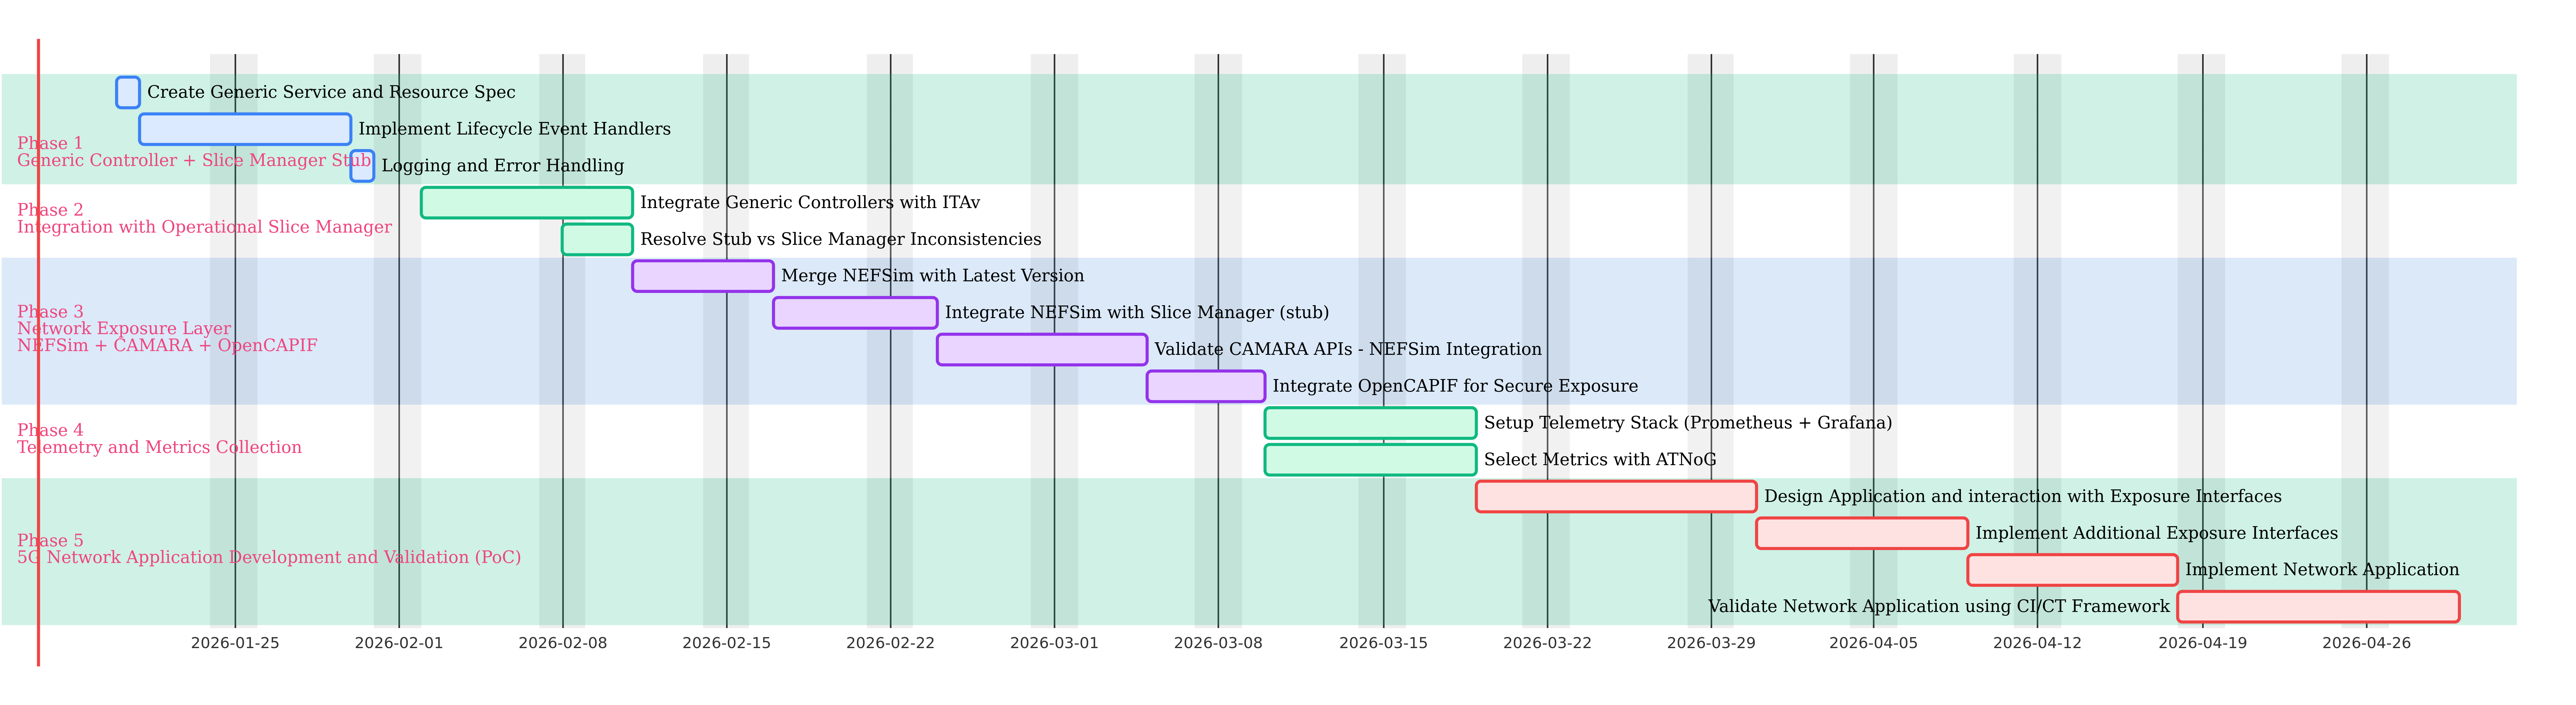
\includegraphics[width=1\linewidth]{figs/gantt_chart.png}
    \caption{Implementation Plan}
    \label{fig:ggant}
\end{figure}
\end{landscape}

The first phase of the implementation plan focuses on Generic Controllers for automated lifecycle management of network slices and \acsp{UE}. The controllers are initially integrated with a Slice Manager stub, providing a simulated interface of the provisioning capabilities of the \acs{ITAv} Slice Manager. This method is adopted to prevent any adverse impact or service disruption on the actual deployed \acs{ITAv} Slice Manager. This phase includes the design of a generic service and resource specification, including lifecycle event handlers for creation, modification, and deletion of slices and \acsp{UE}, all integrated with \acs{OSL}. Logging and error handling support should also be incorporated. As highlighted in Section \ref{chap:proposal:preliminary}, the development of the Slice Manager stub, along with the integration of the slice creation event handler have already been implemented in this first semester.


Following the initial validation with the stub, the generic controller implementations will be integrated with the operational \acs{ITAv} Slice Manager, enabling direct interaction with the 5G system infrastructure. This migration will ensure that the generic controllers can manage network slices and \acs{UE} resources in a fully operational environment. This will allow network application developers to provision and orchestrate their own network slices catered to their use case specific requirements, where they can test their network applications. This phase also includes resolving any possible inconsistencies between the stub and the the \acs{ITAv} Slice Manager, as the author didn't have access to its source code due to its proprietary nature.

Subsequently, the network exposure layer will be implemented. This phase is heavily tied to a previous \acs{ITAv} project, which integrates the following CAMARA/\acs{GSMA} Open Gateway \acsp{API} with the NEFSim~\cite{GSMANEFprojectIT}: \acs{SMS} \acs{OTP}, \acs{QoS} Profiles, Location, \acs{QoD} Provisioning, \acl{QoD}, Geofencinc Subscriptions, Device Reachability Status and Device Roaming Status. However, the given project involves the NEFSim emulating the complete network environment, thereby necessitating integration with the operational \acs{5G} system. This requires: (i) merging the project's NEFSim implementation with its latest version, (ii) integrate the NEFSim to forward all slicing related requests to the slice manager (stub), and (iii) validate the integration of the CAMARA \acsp{API} with the NEFSim, considering certain limitations encountered during this semester as well as new ones that may appear. Afterwards, the NEFSim and the CAMARA \acsp{API} must be integrated with OpenCAPIF for secure exposure. After completing this step, the testbed will enable network app developers with the necessary network interfaces, i.e. \acs{NEF} and CAMARA \acsp{API}, to interact with the network, build their applications, and orchestrate network slices and \acsp{UE}.

In the next phase, the focus is placed on monitoring and logging capabilities within the \acs{5G} network, enabling the exposure of the collected data through well-defined interfaces. To this end, Prometheus exporters are utilized for data collection, with Grafana being employed for visualization and analysis. These metrics play a critical role in the development and validation of networks applications, providing a view of the operational state and performance of the \acs{5G} network. From the metrics collected in Section \ref{sec:testingandvalidation} summarized on Table \ref{tab:metrics:all}, the following metrics of interest were selected for the validations scenarios due to their relevance in assessing operational conditions: \acs{UL}/\acs{DL} throughput, \acs{E2E} latency, \acs{CPU}, memory, \acs{RTT}, jitter, packet loss. This stage requires a deliberation phase with the \acf{ATNoG} to confirm the feasibility of collecting such  metrics.

At this step, the necessary conditions are gathered for the development of network applications, providing developers with: (i) access to the required network interfaces to interact with the network, (ii) provisioning and orchestration capabilities of \acsp{UE} and network slices tailored to their specific use case requirements, where they can deploy and actively test their applications, and (iii) the collection and exposure of network metrics to monitor and evaluate network and application performance. Therefore, a \acs{5G} Network Application will be developed as a \acs{PoC}, leveraging the implemented northbound \acsp{API} or additional \acsp{API} developed as required by the specific use case. This step encompasses the full design, implementation and validation of the network application and required exposure interfaces, ending with its provisioning as an \acs{OSL} service and evaluation via the \acs{CI}/\acs{CT} framework.


